\chapter{Implementation Part I: The Column Store}
\label{chap:Implementation Part I: The Column Store}
% Tell how we want to reduce memory and how database technology comes to the rescue
For the first part of this thesis, our goal is to reduce memory footprint such that client memory requirements can be relaxed. Reduced memory usage are also likely to increase performance due to increased data locality and the cost of memory management. Inspired by the challenges with the current solution which we saw in Section \ref{sec:Challenges with the current solution}, we proceed to use techniques from the field of Database Technology to reduce memory footprint and increase data locality.

% Tell why we pick a column store 
We choose to implement a column store. The reason for this is two-fold. First, as we saw in Section \ref{sub:Row Stores Vs Column Stores}, columns are inherently more compressible. Column stores is, hence, better suited to test our hypothesis and reduce memory footprint than a row-store. Second, the cases where \genus~has experienced performance issues are in situations where a column store is better suited than a row store, for instance on lookup index generation and filter operations.

% Tell why we didn't pick a row store
We believe that transactional processing, where a row store is more suited, will not suffer from using a column-store. On create, update, and delete operations, there constraint checks, validation and memory operations that will make the overhead looking up in multiple columns neglible. Last, row stores mighht rely on indexes that are costly to maintain. Column-stores normally do not need such indexes, because operations on entire columns are efficient \cite{Plattner2014-fr}


\section{CompositionValueCollection}
\label{sec:CompositionValueCollection}
% Lineout the challenges
As we saw in Section \ref{Challenges in Genus App Platform}, one of the challenges in \gap~is the \cn{CompositionObjectValueCollection} class that not only holds the data belonging to each object, but also pointers to the data descriptors. Although this class is flexible because it is self-contained, and can be passed among objects to copy values, for most cases, references to the data descriptors does not generally need to be stored per data collection. 

% Conceptually what is done
\begin{figure}
    \centering
    \begin{subfigure}{1.0\textwidth}
        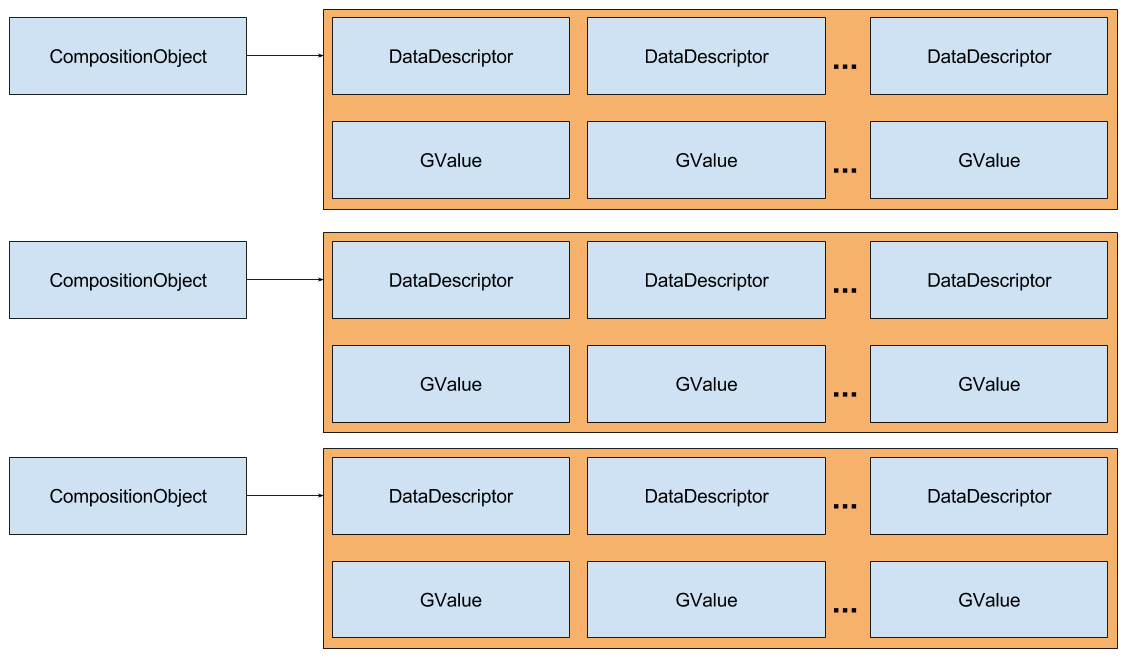
\includegraphics[width=\textwidth]{img/gap-original-rows.png}
        \caption{Original implementation with \cn{CompositionObjectValueColletion}. Each object has its own value collection structure, and each value collection contains pointers to the data descriptors and to the data.}
        \label{fig:gap-original-rows}
    \end{subfigure}
    \begin{subfigure}{1.0\textwidth}
        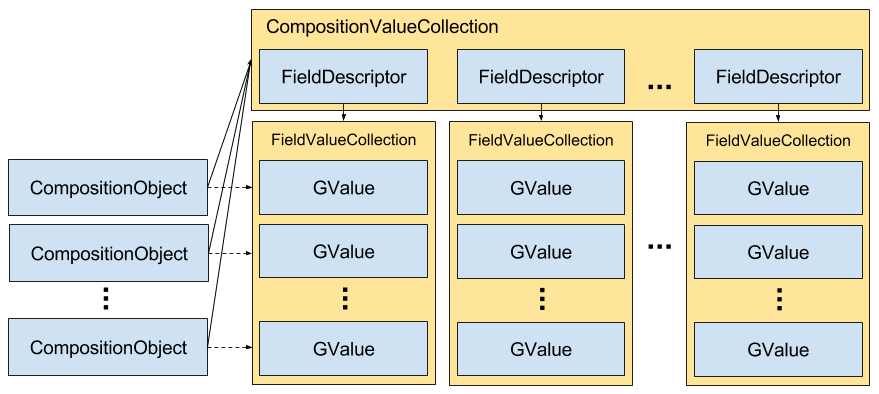
\includegraphics[width=\textwidth]{img/gap-bb-columns.png}
        \caption{Column store implementation with \cn{CompositionValueColletion} and \cn{FieldValueCollection}. All objects in a data source point to the same value collection, and access data using its \cn{DatasourceIndex} which indicates the row number in the columns}
        \label{fig:gap-bb-columns}
    \end{subfigure}
    \caption{Comparison of the original implementation and the column store implementation.}
    \label{fig:gap-storage-comparison}
\end{figure}
In our column store, we plan to replace the \cn{CompositionObjectValueCollection} pointer in each \cn{CompositionObject} with a pointer to a \cn{CompositionValueCollection} and an integer, \cn{DatasourceIndex}, that indicates which position in the data source the object has. All objects within a data source has a pointer to the same \cn{CompositionValueCollection}. This means that composition objects no longer will query its own data collection for values, but rather one common data collection used by all objects. To access a certain value, both \cn{DataDescriptor} and \cn{DatasourceIndex} is required to indicate column and row respectively. A comparison of the old and the new implementation is seen in \ref{fig:gap-storage-comparison}.

% How it impacts memory
In Section \ref{sub:Excessive Amount Of Pointers}, we saw how a data source with objects with 15 properties each needed 32 pointers, or 256 bytes, per objects just for data and data access. Now, this number is reduced to 17 pointers and an integer, which is 140 bytes. Hence, we save 45\% memory by using our new system.

% CompositionObjectValueCollection still exists
Even though the original \cn{CompositionObjectValueCollection} was discarded as the main storage structure, composition objects can still assemble such structures by querying the \cn{CompositionValueCollection}. This is used in object cloning and to transfer data across different data sources in different parts of the application \todo{Stemmer dette?}.

% class diagram
% explain the dictionary and the list of data descriptors
\afigure{img/CompositionValueCollection.png}{\cn{CompositionValueCollection} class diagram.}{fig:CompositionValueCollection}{0.9}
The \cn{CompositionValueCollection} is a class type. The class diagram is shown in Figure \ref{fig:CompositionValueCollection}.

The main methods in the \cn{CompositionValueCollection} class is the \fn{setValue} and \fn{getValue} methods. These functions respectivel set and get \cn{GValues} for a data descriptor and a datasource index. In these operations, the correct column, or \cn{FieldValueCollection}, is looked up in a dictionary, and the index is passed along to the column to get or set the value. If no column exist for a data descriptor, it is created. \fn{isAssigned} and \fn{unassignValue} works similarly. We study the unassigned semantic in Section \ref{sub:Unassigned Values}. 

Datasource indexes are assigned by passing composition objects to the  \fn{registerObject} function. A private variable \vn{maxDatasourceIndex} is used to keep track on the maximum index handed out so far. When an object is received, this variable is incremented and the object is assigned that value. In addition to this, a bitmap \fn{assignedIndexes} is kept to bookkeep which indexes has objects connected to them. When \fn{removeObject} is called, the bit for that index is unset in \fn{assignedIndexes}. In addition, all values corresponding to that object are unassigned. Currently, the \fn{assignedIndexes} bitmap is not used to lookup the first available bit, since this triggers a linear search on every insertion. We discuss this further in the chapter conclusion.

In addition to the above methods, a \cn{CompositionValueCollection} has the ability to unassign an entire row or column by passing in a \cn{CompositionObject} or \cn{DataDescriptor} respectively. We see later in this research where such methods are used.

The \fn{Consolidate} function is called by the data source when it is done loading, and is meant to be an operation where the column store restructures and maximizes space utilization. We see how the columns are affected by this operation in the section about growth strategy, Section \ref{sec:Growth Strategy}.


\section{FieldValueCollection}
\label{sec:FieldValueCollection}

A column is implemented as a \cn{FieldValueCollection} class. This class, uses a \cn{TObjectList<GValue>} to store all values, and all values are accessed using integers. The FieldValueCollection has the following methods:
\begin{itemize}
    \item \fn{Create}
    \item \fn{GetValue}
    \item \fn{SetValue}
    \item \fn{IsAssigned}
    \item \fn{UnassignValue}
\end{itemize}

The basic implementation of \cn{FieldValueCollection} works much like a \cn{TList} type which is built into \delphi, however it has an extra semantic of assigned values.

\subsection{Unassigned Values}
\label{sub:Unassigned Values}
Setting a value to \vn{null} has different semantics than \fn{UnassignValue}. The latter means that there has previously been a value present, but is now removed for performance reasons. This functionality is implemented using a bitmap, \cn{BasicBitArray}, which is based on \delphi~\cn{TBits} type.

\section{Growth Strategy}
\label{sec:Growth Strategy}
Since we used native dynamic arrays, we control the array allocation size. For every reallocation, we risk that the entire array needs to be copied from one part of the memory to another. For this reason, one should be generous when allocating, ideally allocate the correct size immediately. However, since we read a stream of data objects, we are not sure how large our buffers should until the very end. 

\afigure{img/gap-growth-strategy.png}{Growth strategy for buffers. In the load phase, the buffer doubles every time more space is needed. After the load phase, a consolidation is performed which reduces the buffer size to the exact number which are contained in a column.}{fig:gap-growth-strategy}{0.6}
Therefore, we chose a tactic where we double the buffer size every time we need more space. This way, the number of reallocation operations are kept at a minimum. However, this strategy might result in lots of unused buffer space. We, therefore, add a \fn{consolidate} function to our column store that resizes all buffers to fit its data. The strategy is depicted in \ref{gap-growth-strategy}.

\section{Modifiying CompositionObject}
\label{sec:Modifiying CompositionObject}
It must no longer ask its value collection, it must send itself and its datasource index into the GetValue. It no longer holds ownership to a collection, it has a pointer to a value collection shared by all composition objects.

\section{Test results}
\label{sec:Test results}
To test the new implementation, we ran the TPC-H benchmark Q1. 

\subsection{TPC-H Result}
\label{sub:TPC-H Result}

\subsection{Write test results}
\label{sub:Write test results}

\section{Chapter Conclusion}
\label{sec:Chapter Conclusion}


\subsection{Future Work}
\label{sub:Future Work}
Now, we only assign new datasource indexes by incrementing, however we have put in a bitmap for assigned flags. We have disregarded this structure due to the linear search to find the first open bit, and that neither of our benchmarks inserts and removes certain objects. Future work might investigate the effects of using \fn{OpenBit}, and perhaps separate between loading and normal state.

